\chapter{Despliegue}
    En este capítulo se detalla como, una vez terminada una versión final de la aplicación, se comienza con el proceso de habilitar el uso de la aplicación desde la web. Para ello decidimos utilizar la pataforma Hostinger\cite{hostinger}, y todos los servicios que la misma proporciona a sus usuarios.
    \newline
    
    El despliegue de la aplicación consta de tres partes; el despliegue de la aplicación FrontEnd, el despliegue de la aplicación BackEnd, y el despliegue de la base de datos.
    
    \section{FrontEnd}
    Para desplegar la aplicación Angular que representa el FrontEnd de nuestra aplicación, se utilizó la herramienta ``Administrador de archivos'' que nos ofrece Hostinger y que nos proporciona una interfaz de usuario para administrar archivos y directorios en nuestro dominio \textit{tfg-estudio-medico.com}.
    \newline
    
    En dicho administrador, se procedió a subir la carpeta \textit{dist} generada por el proyecto Angular.
    
     \begin{figure}[h]
    \centering
     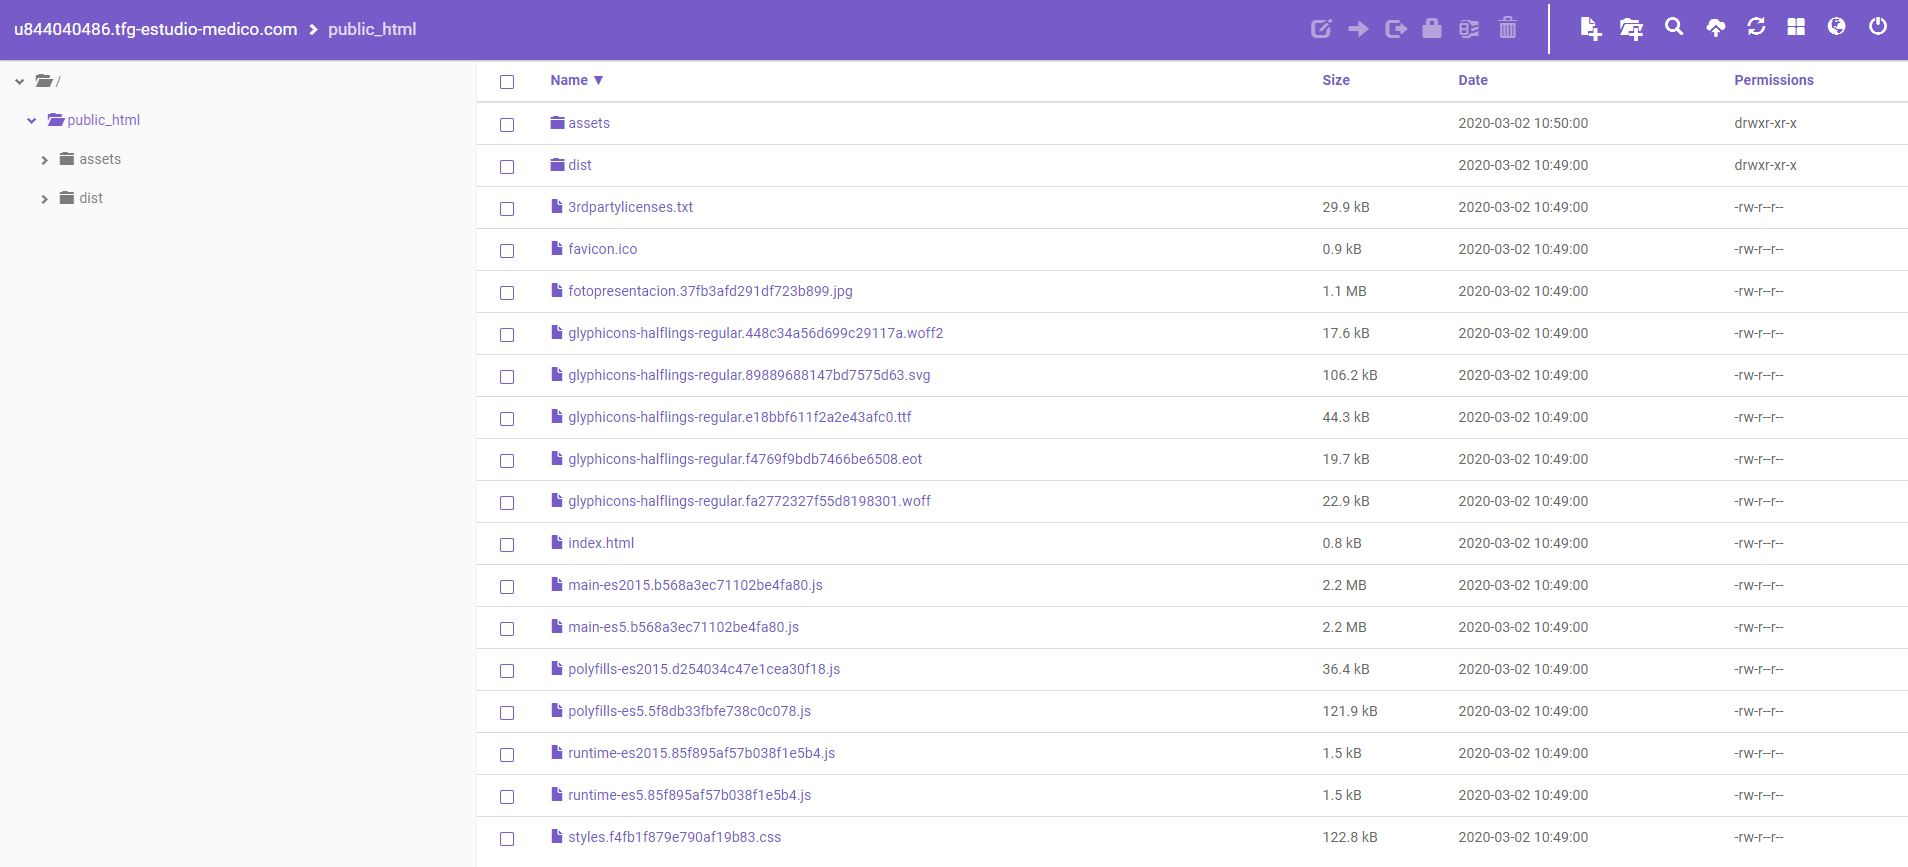
\includegraphics[width=1\textwidth]{images/administradorarchivos}
    \caption{Administrador de archivos de Hostinger}
    \end{figure}
    

    \section{BackEnd}
    Para desplegar la aplicación Java Spring que constituye el BackEnd de nuestra aplicación, se utilizó un servidor proporcionado por Hostinger\cite{hostinger}. En dicho servidor instalamos un sistema operativo Ubuntu 18.04 64bit.
    
     \begin{figure}[h]
    \centering
     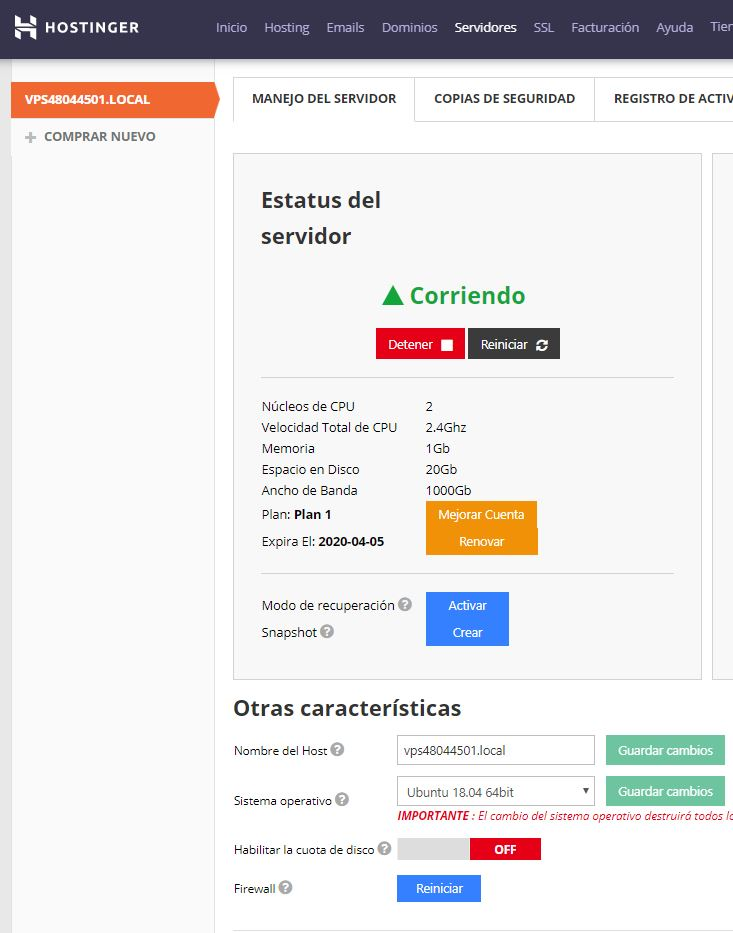
\includegraphics[width=0.5\textwidth]{images/servidorhostinger}
    \caption{Servidor en Hostinger}
    \end{figure}
    
    \FloatBarrier
    
    Para conectarnos al servidor utilizamos el programa MobaXterm, conectándonos al servidor a traves de SSH. Nuestro objetivo era mantener el archivo .jar ejecutándose en la máquina incluso si no estamos conectados a la misma, para ello generamos un \textit{servicio}, esto es, un script que se mantiene arrancado incluso si cerramos la sesión. \\
    \newline
    Una vez generado el archivo SNAPSHOT .jar de nuestro proyecto Java Spring 
    



    
    \section{Base de Datos}
    Para desplegar la base de datos en la web, se utilizó un servicio que ofrece Hostinger para desplegar bases de datos MySQL. 
    \newline 
    A través de PhpMyAdmin y con la opción de generar la base de datos automáticamente al ejecutar un proyecto Java Spring con JPA, se generó la siguiente base de datos:
    
     \begin{figure}[h]
    \centering
     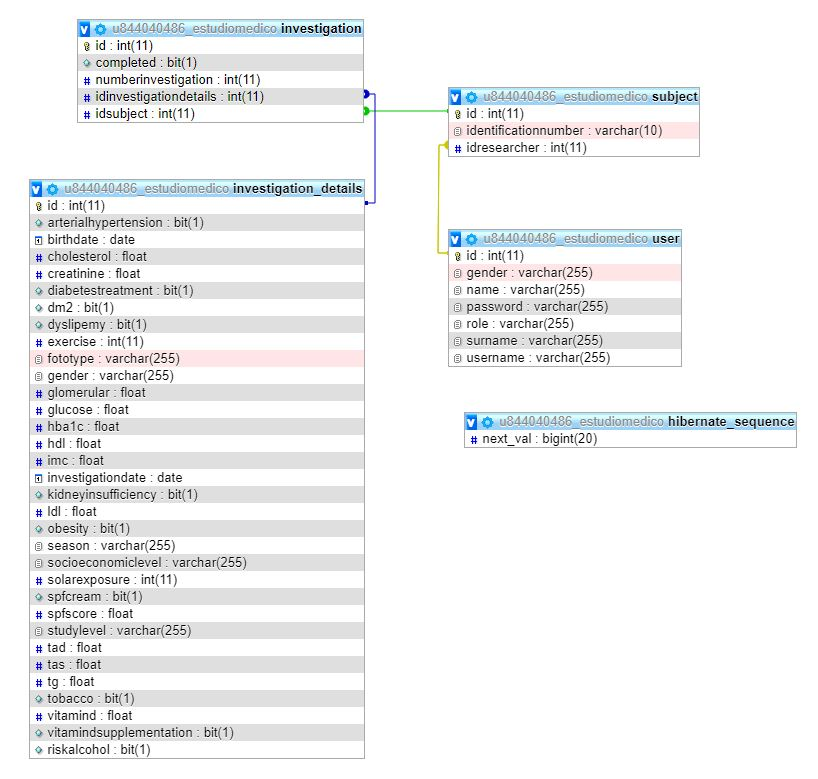
\includegraphics[width=1\textwidth]{images/modelodatos}
    \caption{Modelo de datos generado en PhpMyAdmin}
    \end{figure}
    
    
